\documentclass[11pt,a4paper]{article}
\usepackage[hyperref]{emnlp-ijcnlp-2019}
\usepackage{breakurl}
\usepackage{times}
\usepackage{latexsym}

\usepackage{booktabs}

\usepackage{url}

\usepackage{amsmath}
\usepackage{multirow}
\usepackage{adjustbox}

\usepackage{graphicx}  \usepackage{amsfonts}
\usepackage{subcaption}
\renewcommand{\vec}[1]{\mathbf{#1}} \DeclareMathOperator*{\argmin}{arg\,min}
\DeclareMathOperator*{\argmax}{arg\,max}
\DeclareMathOperator*{\len}{len}
\usepackage{footnote}
\usepackage{epstopdf}
\usepackage{algorithm} \usepackage{algpseudocode} \usepackage{stmaryrd}
\usepackage{booktabs,arydshln}

\usepackage{makecell}
\usepackage{color}
\usepackage{tikz}
\usepackage{pgf}
\usepackage{pgfplots}
\usepackage{tikz-qtree}
\usetikzlibrary{arrows,decorations.pathmorphing,backgrounds,positioning,fit,petri,shapes.misc, arrows.meta,shapes.geometric,decorations.markings,calc,shadows.blur,decorations.pathreplacing,quotes,matrix,shapes.symbols}
\definecolor{fontgray}{RGB}{44, 62, 80}
\definecolor{myred}{RGB}{235, 47, 6} \definecolor{summertime}{RGB}{245, 205, 121}
\definecolor{darkgrass}{RGB}{0, 148, 50}
\definecolor{myblue}{RGB}{0, 168, 255}
\definecolor{mygray}{RGB}{158, 158, 158}
\definecolor{puffin}{RGB}{250, 152, 58}
\definecolor{lowpurple}{RGB}{210, 180, 222}
\definecolor{lowblue}{RGB}{102,178,255}
\definecolor{lowred}{RGB}{245, 183, 177}
\definecolor{darkblue}{rgb}{0, 0, 0.5}

\def\pnode [#1]#2{
\node[regular polygon,regular polygon sides=4, minimum size=1pt,fill=gray,#1, inner sep = 1.2pt] (#2) {};
} 
\tikzset{middlefactor/.style={decoration={
			markings,
			mark= at position #1 with {\pnode[]{}} 
		},postaction={decorate}},
	middlefactor/.default=0.5
}

\newcommand{\squishlist}{
	\begin{list}{}
		{ \setlength{\itemsep}{0pt}
			\setlength{\parsep}{3pt}
			\setlength{\topsep}{3pt}
			\setlength{\partopsep}{0pt}
			\setlength{\leftmargin}{1.5em}
			\setlength{\labelwidth}{1em}
			\setlength{\labelsep}{0.5em} } }
	
	
	\newcounter{Lcount}
	\newcommand{\squishlisttwo}{
		\begin{list}{\arabic{Lcount}. }
			{ \usecounter{Lcount}
				\setlength{\itemsep}{0pt}
				\setlength{\parsep}{0pt}
				\setlength{\topsep}{0pt}
				\setlength{\partopsep}{0pt}
				\setlength{\leftmargin}{2em}
				\setlength{\labelwidth}{1.5em}
				\setlength{\labelsep}{0.5em} } }
		
		\newcommand{\squishend}{
	\end{list} }

\makeatletter
\def\adl@drawiv#1#2#3{\hskip.5\tabcolsep
	\xleaders#3{#2.5\@tempdimb #1{1}#2.5\@tempdimb}#2\z@ plus1fil minus1fil\relax
	\hskip.5\tabcolsep}
\newcommand{\cdashlinelr}[1]{\noalign{\vskip\aboverulesep
		\global\let\@dashdrawstore\adl@draw
		\global\let\adl@draw\adl@drawiv}
	\cdashline{#1}
	\noalign{\global\let\adl@draw\@dashdrawstore
		\vskip\belowrulesep}}
\def\blfootnote{\xdef\@thefnmark{}\@footnotetext}
\makeatother

\aclfinalcopy 



\newcommand\BibTeX{B{\sc ib}\TeX}
\newcommand\confname{EMNLP-IJCNLP 2019}
\newcommand\conforg{SIGDAT}

\title{Dependency-Guided LSTM-CRF for Named Entity Recognition}

\author{Zhanming Jie \and Wei Lu\\
  StatNLP Research Group\\
  Singapore University of Technology and Design \\
\texttt{zhanming\_jie@mymail.sutd.edu.sg, luwei@sutd.edu.sg} \\}


\date{}

\begin{document}
\maketitle
\begin{abstract}
Dependency tree structures capture long-distance and syntactic relationships between words in a sentence.  
  The syntactic relations (e.g., {\it nominal subject}, {\it object}) can potentially infer the existence of certain named entities. 
  In addition, the performance of a named entity recognizer could benefit from the long-distance dependencies between the words in dependency trees. 
  In this work, we propose a simple yet effective {\it dependency-guided} LSTM-CRF model to encode the complete dependency trees and capture the above properties for the task of named entity recognition (NER).
The data statistics show strong correlations between the entity types and dependency relations.
  We conduct extensive experiments on several standard datasets and demonstrate the effectiveness of the proposed model in improving NER and achieving state-of-the-art performance. 
Our analysis reveals that the significant improvements mainly result from the dependency relations and long-distance interactions provided by dependency trees.


\end{abstract}

\section{Introduction}
\label{sec:intro}
\blfootnote{Accepted as a long paper in EMNLP 2019 (Conference on Empirical Methods in Natural Language Processing).}
Named entity recognition (NER) is one of the most important and fundamental tasks in natural language processing (NLP).
Named entities capture useful semantic information which was shown helpful for downstream NLP tasks such as coreference resolution~\cite{lee2017end}, relation extraction~\cite{miwa2016end} and semantic parsing~\cite{dong2018coarse}.
On the other hand, dependency trees also capture useful semantic information within natural language sentences. 
Currently, research efforts have derived useful discrete features from dependency structures~\cite{sasano2008japanese,cucchiarelli2001unsupervised,ling2012fine} or structural constraints~\cite{jie2017efficient} to help the NER task. 
However, how to make good use of the rich relational information as well as complex long-distance interactions among words as conveyed by the complete dependency structures for improved NER remains a research question to be answered.


\begin{figure}[t!]
	\centering
\adjustbox{max width=1.0\linewidth}{
	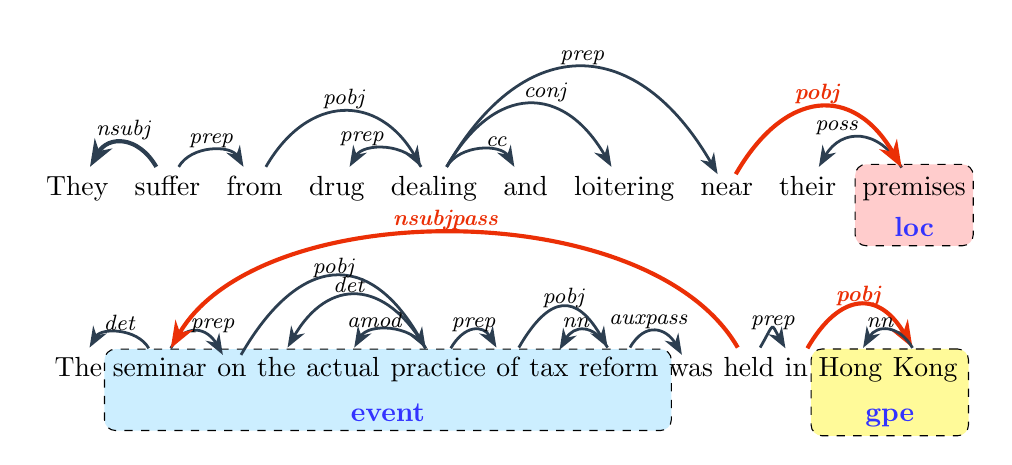
\begin{tikzpicture}[node distance=1.0mm and 1.0mm, >=Stealth, 
		wordnode/.style={draw=none, minimum height=5mm, inner sep=0pt},
		chainLine/.style={line width=1pt,-, color=fontgray},
		entbox/.style={draw=black, rounded corners, fill=red!20, dashed}
		]
\matrix (sent1) [matrix of nodes, nodes in empty cells, execute at empty cell=\node{\strut};]
		{
		 They & [1mm]suffer &[1mm]from & [1mm]drug   &  [1mm]  dealing & [1mm]and& [1mm]loitering& [1mm]near & [1mm]their & [1mm]premises\\
};
	
		\draw [chainLine, ->, color=fontgray, line width=1.5pt] (sent1-1-2) to [out=120,in=60, looseness=1.4] node[above, yshift=-1mm, color=black]{\footnotesize\it nsubj} (sent1-1-1);
		\draw [chainLine, ->] (sent1-1-2) to [out=60,in=120, looseness=1] node[above, yshift=-1mm, color=black]{\footnotesize\it prep} (sent1-1-3);
		\draw [chainLine, ->] (sent1-1-5) to [out=120,in=60, looseness=1] node[above, yshift=-1mm, xshift=-3mm, color=black]{\footnotesize\it prep} (sent1-1-4);
		\draw [chainLine, ->] (sent1-1-3) to [out=60,in=120, looseness=1.4] node[above, yshift=-1mm, color=black]{\footnotesize\it pobj} (sent1-1-5);
		\draw [chainLine, ->] (sent1-1-5) to [out=60,in=120, looseness=1] node[above, yshift=-1mm, color=black, xshift=2mm]{\footnotesize\it cc} (sent1-1-6);
		\draw [chainLine, ->] (sent1-1-5) to [out=60,in=120, looseness=1.5] node[above, yshift=-1mm, color=black, xshift=2mm]{\footnotesize\it conj} (sent1-1-7);
		\draw [chainLine, ->] (sent1-1-5) to [out=60,in=120, looseness=1.5] node[above, yshift=-1mm, color=black]{\footnotesize\it prep} (sent1-1-8);
		\draw [chainLine, ->, color=fontgray, line width=1pt] (sent1-1-10) to [out=120,in=60, looseness=1.4] node[above, yshift=-1mm, color=black, xshift=-3mm]{\footnotesize\it poss} (sent1-1-9);
		\draw [chainLine, ->, line width=1.5pt, color=myred] (sent1-1-8) to [out=60,in=120, looseness=1.5] node[above, yshift=-1mm, color=myred]{\footnotesize\textit{\textbf{pobj}} } (sent1-1-10);
		
		\begin{pgfonlayer}{background}
		\node [entbox, below=of sent1-1-10, yshift=7mm, text height=8mm, minimum width=15mm] (e1)  [] {\color{blue!80}\textbf{\textsc{loc}}};
\end{pgfonlayer}
		
		
		
		\matrix (sent2) [matrix of nodes, nodes in empty cells, execute at empty cell=\node{\strut};, below=of sent1, yshift=-14mm]
		{
			The &[-1mm] seminar &[-1mm] on &[-1mm] the & [-1mm]actual   &    [-1mm]practice &[-1mm] of & [-1mm]tax& [-1mm]reform & [-1mm]was & [-1mm]held & [-1mm]in &[-1mm] Hong &[-1mm] Kong\\
};
	
		\draw [chainLine, ->] (sent2-1-2) to [out=120,in=60, looseness=1] node[above, yshift=-1mm, xshift=0mm,  color=black]{\footnotesize\it det} (sent2-1-1);
		\draw [chainLine, <-] (sent2-1-3) to [out=120,in=60, looseness=1.5] node[above, yshift=-1.5mm,  color=black, xshift=2mm]{\footnotesize\it prep} (sent2-1-2);
		\draw [chainLine, ->] (sent2-1-6) to [out=120,in=60, looseness=1.5] node[above, yshift=-1mm, xshift=-1mm,  color=black]{\footnotesize\it det} (sent2-1-4);
		\draw [chainLine, ->] (sent2-1-6) to [out=120,in=60, looseness=1] node[above, yshift=-1mm, xshift=-2mm,  color=black]{\footnotesize\it amod} (sent2-1-5);
		\draw [chainLine, ->] (sent2-1-3) to [out=60,in=120, looseness=1.6] node[above, yshift=-1.5mm,  color=black]{\footnotesize\it pobj} (sent2-1-6);
		\draw [chainLine, ->] (sent2-1-6) to [out=60,in=120, looseness=1.5] node[above, yshift=-1.5mm,  color=black]{\footnotesize\it prep} (sent2-1-7);
		\draw [chainLine,<-, line width=1pt] (sent2-1-8) to [out=60,in=120, looseness=1.5] node[above, yshift=-1mm, color=black,xshift=-1mm]{\footnotesize\it nn} (sent2-1-9);
		\draw [chainLine, ->] (sent2-1-7) to [out=60,in=120, looseness=1.8] node[above, yshift=-1.5mm,  color=black]{\footnotesize\it pobj} (sent2-1-9);
		
		\draw [chainLine,->, line width=1pt] (sent2-1-9) to [out=60,in=120, looseness=1.5] node[above, yshift=-1mm, color=black,xshift=-1mm]{\footnotesize\it auxpass} (sent2-1-10);
		\draw [chainLine, ->] (sent2-1-11) to [out=60,in=120, looseness=3.0] node[above, yshift=-1.5mm,  color=black]{\footnotesize\it prep} (sent2-1-12);
		
		\draw [chainLine, ->, color=myred, line width=1.5pt] (sent2-1-12) to [out=60,in=120, looseness=1.6] node[above, yshift=-1.5mm,  color=myred]{\footnotesize\textit{\textbf{pobj}}} (sent2-1-14);
		\draw [chainLine, <-] (sent2-1-13) to [out=60,in=120, looseness=1.4] node[above, yshift=-1mm,  color=black, xshift=-1mm]{\footnotesize\it nn} (sent2-1-14);
		
		\draw [chainLine, <-, color=myred, line width=1.5pt] (sent2-1-2) to [out=60,in=120, looseness=0.8] node[above, yshift=-1mm,  color=myred, xshift=-1mm]{\footnotesize\textit{\textbf{nsubjpass}}} (sent2-1-11);
		
	
		\begin{pgfonlayer}{background}
		\node [entbox, below=of sent2-1-5, xshift=5.7mm, yshift=5.8mm, text height=8mm, minimum width=72mm, fill=myblue!20] (e2)  [] {\color{blue!80}\textbf{\textsc{event}}};
		\node [entbox, below=of sent2-1-13, xshift=5mm, yshift=6.5mm, text height=8mm, minimum width=20mm, fill=yellow!40] (e2)  [] {\color{blue!80}\textbf{\textsc{gpe}}};
		\end{pgfonlayer}
	\end{tikzpicture} 
	}
\caption{Example sentences annotated with named entiteis and dependencies in the OntoNotes 5.0 dataset.}
\label{fig:examples}
\end{figure}






The first example in Figure \ref{fig:examples} illustrates the relationship between a dependency structure and a named entity. 
Specifically, the word ``{\it premises}'', which is a named entity of type \textsc{loc} (location), is characterized by the incoming arc with label ``{\it pobj}'' (prepositional object). 
This arc reveals a certain level of the semantic role that the word ``{\it premises}'' plays in the sentence. 
Similarly, the two words ``{\it Hong Kong}'' in the second example that form an entity of type \textsc{gpe} are also characterized by a similar dependency arc towards them.




The long-distance dependencies capturing non-local structural information can also be very helpful for the NER task~\cite{finkel2005incorporating}. 
In the second example of Figure \ref{fig:examples}, the long-distance dependency from ``\textit{held}'' to ``\textit{seminar}'' indicates a direct relation ``\textit{nsubjpass}'' (passive subject) between them, which can be used to characterize the existence of an entity. 
However, existing NER models based on linear-chain structures would have difficulties in capturing such long-distance relations (i.e., non-local structures).

One interesting property, as highlighted in the work of \citet{jie2017efficient}, is that most of the entities form subtrees under their corresponding dependency trees. 
In the example of the \textsc{Event} entity in Figure \ref{fig:examples}, the entity itself forms a subtree and the words inside have rich complex dependencies among themselves. 
Exploiting such dependency edges within the subtrees allows a model to capture non-trivial semantic-level interactions between words within long entities.
For example, ``\textit{practice}'' is the prepositional object (\textit{pobj}) of ``\textit{on}'' which is a preposition (\textit{prep}) of ``\textit{seminar}'' in the \textsc{Event} entity. 
Modeling these grandchild dependencies (GD)~\cite{koo2010efficient} requires the model to capture some higher-order long-distance interactions among different words in a sentence.






Inspired by the above characteristics of dependency structures, in this work, we propose a simple yet effective dependency-guided model for NER. 
Our neural network based model is able to capture both contextual information and rich long-distance interactions between words for the NER task. 
Through extensive experiments on several datasets on different languages, we demonstrate the effectiveness of our model, which achieves the state-of-the-art performance. 
To the best of our knowledge, this is the first work that leverages the complete dependency graphs for NER.
 We make our code publicly available at \url{http://www.statnlp.org/research/information-extraction}.










\section{Related Work}
NER has been a long-standing task in the field of NLP. 
While many recent works~\cite{peters2018deep,akbik2018coling,devlin2019bert} focus on finding good contextualized word representations for improving NER, our work is mostly related to the literature that focuses on employing dependency trees for improving NER. 


\citet{sasano2008japanese} exploited the syntactic dependency features for Japanese NER and achieved improved performance with a support vector machine~(SVM)~\cite{cortes1995support} classifier. 
Similarly, \citet{ling2012fine} included the head word in a dependency edge as features for fine-grained entity recognition. 
Their approach is a pipeline where they extract the entity mentions with  linear-chain conditional random fields~(CRF)~\cite{lafferty2001conditional} and used a classifier to predict the entity type.
\citet{liu2010recognizing} proposed to link the words that are associated with selected typed dependencies (e.g., ``{\it nn}'', ``{\it prep}'') using a skip-chain CRF~\cite{sutton2004collective} model. 
They showed that some specific relations between the words can be exploited for improved NER. 
\citet{cucchiarelli2001unsupervised} applied a dependency parser to obtain the syntactic relations for the purpose of unsupervised NER. 
The resulting relation information serves as the features for potential existence of named entities. 
\citet{jie2017efficient} proposed an efficient dependency-guided model based on the semi-Markov CRF~\cite{sarawagi2004semi} for NER. 
The purpose is to reduce time complexity while maintaining the non-Markovian features.
They observed certain relationships between the dependency edges and the named entities. 
Such relationships are able to define a reduced search space for their model. 
While these previous approaches do not make full use of the dependency tree structures, we focus on exploring neural architectures to exploit the  complete structural information conveyed by the dependency trees.








\section{Model}

Our dependency-guided model is based on the state-of-the-art BiLSTM-CRF model proposed by \citet{lample2016neural}.
We first briefly present their model  as background and next present our dependency-guided model.



\subsection{Background: BiLSTM-CRF}
In the task of named entity recognition, we aim to predict the label sequence  given the input sentence  where  is the number of words.
The labels in  are defined by a label set with the standard \textsc{iobes}\footnote{``\textsc{s-}'' indicates the entity with a single word and ``\textsc{e-}'' indicates the end of an entity.} labeling scheme~\cite{ramshaw1999text,ratinov2009design}. 
The CRF~\cite{lafferty2001conditional} layer defines the probability of the label sequence  given :



Following \citet{lample2016neural}, the score is defined as the sum of transitions and emissions from the bidirectional LSTM (BiLSTM): 

where  is a transition matrix in which  is the transition parameter from the label  to the label \footnote{ and  are \texttt{start} and \texttt{end} labels.}. 
 is an emission matrix where  represents the scores of the label   at the -th position. 
Such scores are provided by the parameterized LSTM~\cite{hochreiter1997long} networks. 
During training, we minimize the negative log-likelihood to obtain the model parameters including both LSTM and transition parameters. 




\subsection{Dependency-Guided LSTM-CRF}
\paragraph{Input Representations}
The word representation  in the BiLSTM-CRF~\cite{lample2016neural,ma2016end,D17-1035} model consists of the concatenation of the word embedding as well as the corresponding character-based representation. 
Inspired by the fact that each word (except the root) in a sentence has exactly one \textit{head} (i.e., \textit{parent}) word in the dependency structure, we can enhance the word representations with such dependency information. 
Similar to the work by \citet{miwa2016end}, we concatenate the word representation together with the corresponding head word representation and dependency relation embedding as the input representation. 
Specifically, given a dependency edge  with  as parent,  as child and  as dependency relation, the representation at position  can be denoted as:

where  and  are the word representations of the word  and its parent , respectively. 
We take the final hidden state of character-level BiLSTM as the character-based representation~\cite{lample2016neural}.
 is the embedding for the dependency relation . 
These relation embeddings are randomly initialized and fine-tuned during training. 
The above representation allows us to capture the direct long-distance interactions at the input layer. 
For the word that is a root of the dependency tree, we treat its parent as itself\footnote{We also tried using a root word embedding but the performance is similar.} and create a root relation embedding. 
Additionally, contextualized word representations (e.g., ELMo) can also be concatenated into .

\begin{figure}[t!]
	\centering
	\adjustbox{max width=1\linewidth}{
		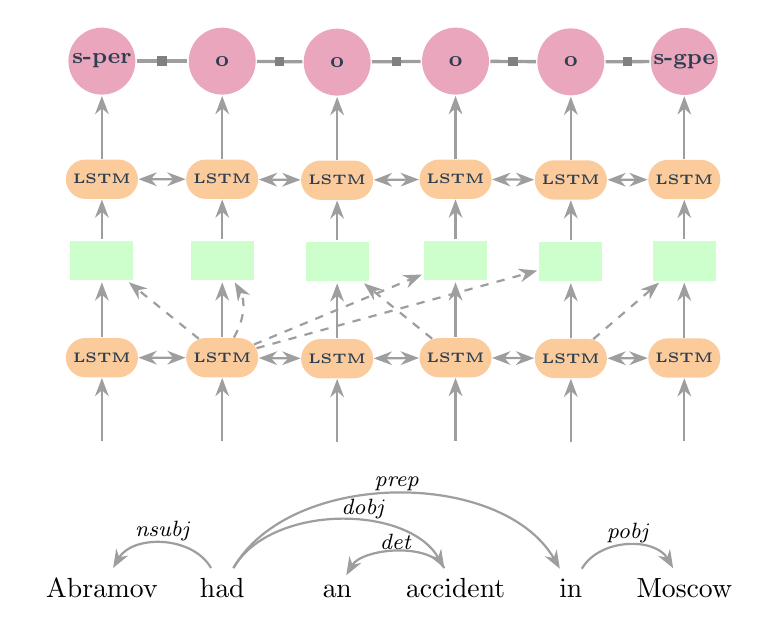
\begin{tikzpicture}[node distance=8.0mm and 10mm, >=Stealth, 
		sentity/.style={draw=none, circle, minimum height=8.5mm, minimum width=8.5mm,line width=1pt, inner sep=0pt, fill=purple!35},
		lstm/.style={draw=none, minimum height=5mm, rounded rectangle, fill=puffin!50, minimum width=11.5mm, label={center:\tiny \textcolor{fontgray}{\bf LSTM}}},
plus/.style={draw=none, minimum height=3mm, circle, fill={rgb:red,0;green,210;blue,211}, label={center:\footnotesize \textcolor{white}{+}}},
		gfunc/.style={draw=none, minimum height=5mm, rectangle, fill=green!20, label={center:\footnotesize \textcolor{fontgray}{}}, minimum width=8mm, line width = 1.5pt},
		emb/.style={draw=none, minimum height=3mm, rounded rectangle, fill=none, minimum width=12mm, text=fontgray},
chainLine/.style={line width=0.8pt,->, color=mygray},
]
		
		
		\matrix (s) [matrix of nodes, nodes in empty cells, execute at empty cell=\node{\strut};]
		{
			Abramov & [2ex]had & [5ex]an & [3ex]accident   &   [3ex] in  & [3ex] Moscow\\
};
		
		\draw [chainLine, ->] (s-1-2) to [out=120,in=60, looseness=1] node[above, yshift=-1mm, color=black]{\footnotesize\it nsubj} (s-1-1);
		\draw [chainLine, ->] (s-1-4) to [out=120,in=60, looseness=0.8] node[above, yshift=-1mm, color=black]{\footnotesize\it det} (s-1-3);
		\draw [chainLine, ->] (s-1-2) to [out=60,in=120, looseness=0.9] node[above, yshift=-1.2mm, xshift=3mm, color=black]{\footnotesize\it dobj} (s-1-4);
		\draw [chainLine, ->] (s-1-2) to [out=60,in=120, looseness=0.9] node[above, yshift=-1mm, color=black]{\footnotesize\it prep} (s-1-5);
		\draw [chainLine, ->] (s-1-5) to [out=60,in=120, looseness=1] node[above, yshift=-1mm, color=black]{\footnotesize\it pobj} (s-1-6);
		
		\node[emb, above= of s-1-1, yshift=5mm] (u1) {};
		\node[emb, above= of s-1-2, yshift=5mm] (u2) {};
		\node[emb, above= of s-1-3, yshift=5.8mm] (u3) {};
		\node[emb, above= of s-1-4, yshift=5mm] (u4) {};
		\node[emb, above= of s-1-5, yshift=5mm] (u5) {};
		\node[emb, above= of s-1-6, yshift=5mm] (u6) {};
		
		\node[lstm, above= of u1] (h1) {};
		\node[lstm, above=of u2](h2) {};
		\node[lstm, above= of u3](h3) {};
		\node[lstm, above= of u4](h4) {};
		\node[lstm, above= of u5](h5) {};
		\node[lstm, above= of u6](h6) {};
		
		
		
		\node[gfunc, above= of h1, yshift=-1mm] (g1) {};
		\node[gfunc, above=of h2, yshift=-1mm](g2) {};
		\node[gfunc, above= of h3, yshift=-1mm](g3) {};
		\node[gfunc, above= of h4, yshift=-1mm](g4) {};
		\node[gfunc, above= of h5, yshift=-1mm](g5) {};
		\node[gfunc, above= of h6, yshift=-1mm](g6) {};
		
		\node[lstm, above= of g1, yshift=-3mm] (m1) {};
		\node[lstm, above=of g2, yshift=-3mm](m2) {};
		\node[lstm, above= of g3, yshift=-3mm](m3) {};
		\node[lstm, above= of g4, yshift=-3mm](m4) {};
		\node[lstm, above= of g5, yshift=-3mm](m5) {};
		\node[lstm, above= of g6, yshift=-3mm](m6) {};
		


		\node[sentity, above= of m1] (e1) {\footnotesize \textcolor{fontgray}{\bf \textsc{s-per}}};
		\node[sentity, above=of m2](e2) {\footnotesize \textcolor{fontgray}{\bf \textsc{o}}};
		\node[sentity, above= of m3](e3) {\footnotesize \textcolor{fontgray}{\bf \textsc{o}}};
		\node[sentity, above= of m4](e4) {\footnotesize \textcolor{fontgray}{\bf \textsc{o}}};
		\node[sentity, above= of m5](e5) {\footnotesize \textcolor{fontgray}{\bf \textsc{o}}};
		\node[sentity, above= of m6](e6) {\footnotesize \textcolor{fontgray}{\bf \textsc{s-gpe}}};
		
		
		\draw [chainLine] (u1) to (h1);
		\draw [chainLine] (u2) to (h2);
		\draw [chainLine] (u3) to (h3);
		\draw [chainLine] (u4) to (h4);
		\draw [chainLine] (u5) to (h5);
		\draw [chainLine] (u6) to (h6);
		
		\draw [chainLine] (h1) to  (g1);
		\draw [chainLine] (h2) to (g2);
		\draw [chainLine] (h3) to (g3);
		\draw [chainLine] (h4) to (g4);
		\draw [chainLine] (h5) to (g5);
		\draw [chainLine] (h6) to (g6);
		
		\draw [chainLine] (g1) to (m1);
		\draw [chainLine] (g2) to (m2);
		\draw [chainLine] (g3) to (m3);
		\draw [chainLine] (g4) to (m4);
		\draw [chainLine] (g5) to (m5);
		\draw [chainLine] (g6) to (m6);
		
		\draw [chainLine] (m1) to  (e1);
		\draw [chainLine] (m2) to   (e2);
		\draw [chainLine] (m3) to   (e3);
		\draw [chainLine] (m4) to    (e4);
		\draw [chainLine] (m5) to   (e5);
		\draw [chainLine] (m6) to   (e6);
		
		\draw [chainLine, dashed] (h2) to  [out=60,in=-60] (g2);
		\draw [chainLine, dashed] (h2) to (g1);
		\draw [chainLine, dashed] (h2) to (g4);
		\draw [chainLine, dashed] (h2) to (g5);
		\draw [chainLine, dashed] (h4) to (g3);
		\draw [chainLine, dashed] (h5) to (g6);
		
		\draw [chainLine, <->] (h1) to (h2);
		\draw [chainLine, <->] (h2) to (h3);
		\draw [chainLine, <->] (h3) to (h4);
		\draw [chainLine, <->] (h4) to (h5);
		\draw [chainLine, <->] (h5) to (h6);
		
		\draw [chainLine, <->] (m1) to (m2);
		\draw [chainLine, <->] (m2) to (m3);
		\draw [chainLine, <->] (m3) to (m4);
		\draw [chainLine, <->] (m4) to (m5);
		\draw [chainLine, <->] (m5) to (m6);
		
		\draw [chainLine, line width=1.2pt, -, middlefactor] (e1) to (e2);
		\draw [chainLine, line width=1.2pt, -, middlefactor] (e2)to (e3);
		\draw [chainLine, line width=1.2pt, -, middlefactor] (e3)to (e4);
		\draw [chainLine, line width=1.2pt, -, middlefactor]  (e4)to (e5);
		\draw [chainLine, line width=1.2pt, -, middlefactor] (e5)to (e6);
		
		\end{tikzpicture} 
	}
\caption{Dependency-guided LSTM-CRF with 2 LSTM Layers. Dashed connections mimic the dependency edges. ``'' represents the interaction function.}
\label{fig:model2layer}
\end{figure}




\paragraph{Neural Architecture}
Given the dependency-encoded input representation , we apply the LSTM to capture the contextual information and model the interactions between the words and their corresponding parents in the dependency trees. 
Figure \ref{fig:model2layer} shows the proposed dependency-guided LSTM-CRF (\textbf{DGLSTM-CRF}) with 2 LSTM layers for the example sentence ``\textit{Abramov had an accident in Moscow}'' and its dependency structure. 
The corresponding label sequence is \{\textsc{s-per}, \textsc{o}, \textsc{o}, \textsc{o}, \textsc{o}, \textsc{s-gpe}\}. 
Followed by the first BiLSTM, the hidden states at each position will propagate to the next BiLSTM layer and its child along the dependency trees. 
For example, the hidden state of the word ``\textit{had}'', , will propagate to its child ``\textit{Abramov}'' at the first position. 
For the word that is root, the hidden state at that specific position will propagate to itself. 
We use an \textit{interaction function}  to capture the interaction between the child and its parent in a dependency. 
Such an interaction function can be concatenation, addition or a  multilayer perceptron (MLP). 
We further apply another BiLSTM layer on top of the interaction functions to produce the context representation for the final CRF layer. 

The architecture shown in Figure \ref{fig:model2layer} with a 2-layer BiLSTM can effectively encode the grandchild dependencies because the input representations encode the parent information and the interaction function further propagate the grandparent information. 
Such propagations allow the model to capture the indirect long-distance interactions from the grandchild dependencies between the words in the sentence as mentioned in Section \ref{sec:intro}. 
In general, we can stack more interaction functions and BiLSTMs to enable deeper reasoning over the dependency trees. 
Specifically, the hidden states of the -th layer  can be calculated from the hidden state of the previous layer :

where  indicates the parent index of the word . 
 represents the interaction functions between the hidden state at the -th and  -th positions under the dependency edges . 
The number of layers  can be chosen according to the performance on the development set. 

\begin{table}[t!]
	\centering
	\scalebox{0.8}{
		\begin{tabular}{ll}
			\toprule
			\textbf{Interaction Function}&  \\
			\midrule
			Self connection & \\
			Concatenation & \\
			Addition & \\
			MLP &  \\
			\bottomrule
		\end{tabular}
	}
\caption{List of interaction functions.}
\label{tab:interfunc}
\end{table}

\paragraph{Interaction Function}
The interaction function between the parent and child representations can be defined in various ways. 
Table \ref{tab:interfunc} shows the list of interaction function considered in our experiments. 
The first one returns the hidden state itself, which is equivalent to stacking the LSTM layers. 
The concatenation and addition involve no parameter, which are straightforward ways to model the interactions. 
The last one applies an MLP to model the interaction between parent and child representations. 
With the rectified linear unit (ReLU) as activation function, the  function is analogous to a graph convolutional network (GCN)~\cite{kipf2017semi} formulation. 
In such a graph, each node has a self connection (i.e., ) and a dependency connection with parent (i.e., ).  
Similar to the work by \citet{marcheggiani2017encoding}, we adopt different parameters  and  for self and dependency connections. 








\section{Experiments}




\paragraph{Datasets}
The main experiments are conducted on the large-scale OntoNotes 5.0~\cite{weischedel2013ontonotes} English and Chinese datasets.
We chose these datasets  because  they contain both constituency tree and named entity annotations. 
There are 18 types of entities defined in the OntoNotes dataset. 
We convert the constituency trees into the Stanford dependency~\cite{de2008stanford} trees using the rule-based tool~\cite{de2006generating} by Stanford CoreNLP~\cite{manning2014stanford}.
For English, \citet{pradhan2013towards} provided the train/dev/test split\footnote{http://cemantix.org/data/ontonotes.html} and the split has been used by several previous works~\cite{chiu2016named,li2017leveraging,ghaddar2018robust}.
For Chinese, we use the official splits provided by \citet{pradhan2012conll}\footnote{http://conll.cemantix.org/2012/data.html}.



\begin{table}[t!]
	\centering
	\setlength{\tabcolsep}{2pt} \renewcommand{\arraystretch}{1.1} \resizebox{1.0\linewidth}{!}{
		\begin{tabular}{l cccccccc}
			\toprule
			\multirow{2}{*}{\textbf{Dataset}} & \multicolumn{2}{c}{\bf Train} & \multicolumn{2}{c}{\bf Dev} & \multicolumn{2}{c}{\bf Test} & \textbf{ST} & \textbf{GD} \1mm]
			
			\multicolumn{3}{l}{\textbf{Contextualized Word Representation}} &\\
			\citet{akbik2018coling} (Flair) & - & - & 89.30 \\
			\cdashlinelr{1-4}
			BiLSTM-CRF () + {\footnotesize ELMo} & 85.44& 84.41 & 84.92 \\
			BiLSTM-CRF () + {\footnotesize ELMo} & 89.14 & 88.59 & 88.87 \\
			BiLSTM-CRF  () + {\footnotesize ELMo}  & 88.25 & 89.71 & 88.98 \\
			BiLSTM-CRF () + {\footnotesize ELMo} & 88.03 & 89.04 & 88.53 \\
			
			BiLSTM-GCN-CRF +  {\footnotesize ELMo}   & 89.40 & 89.71 & 89.55 \\
			\cdashlinelr{1-4}
			DGLSTM-CRF () + {\footnotesize ELMo} &86.87  &85.12  &85.99 \\
			DGLSTM-CRF () + {\footnotesize ELMo} & 89.40 & 89.96 & 89.68 \\
			DGLSTM-CRF () + {\footnotesize ELMo} & \textbf{89.59} & \textbf{90.17} & {\bf 89.88} \\
			DGLSTM-CRF () + {\footnotesize ELMo} & 89.43 & 90.15 & 89.79 \\
\bottomrule
		\end{tabular}
	}
\caption{Performance comparison on the OntoNotes 5.0 English dataset.}
\label{tab:mainresults}
\end{table}

We further compare the performance of all models with ELMo~\cite{peters2018deep} representations to investigate whether the effect of dependency would be diminished by the contextualized word representations. 
With  = , the ELMo representations largely improve the performance of BiLSTM-CRF compared to the BiLSTM-CRF model with word embeddings only but is still 1 point below our DGLSTM-CRF model. 
The 2-layer DGLSTM-CRF model outperforms the best BilSTM-CRF baseline with 0.9 points in F ().
Empirically, we found that among the entities that are correctly predicted by DGLSTM-CRF but wrongly predicted by BiLSTM-CRF, 47\% of them are with length more than 2. 
Our finding shows the 2-layer DGLSTM-CRF model is able to accurately recognize long entities, which can lead to a higher precision.  
In addition, 51.9\% of the entities that are correctly retrieved by DGLSTM-CRF have the dependency relations ``\textit{pobj}'', ``\textit{nn}'' and ``\textit{nsubj}'', which have strong correlations with certain named entity types (Figure \ref{fig:depstat}).  
Such a result demonstrates the effectiveness of dependency relations in improving the recall of NER.






\begin{table}
	\centering
	\resizebox{\linewidth}{!}{
		\begin{tabular}{lccc}
			\toprule
			\textbf{Model}& \textbf{Prec.} & \textbf{Rec.} & \textbf{F} \\
			\midrule
			\citet{pradhan2013towards}  &78.20 & 66.45 & 71.85\\ 
Lattice LSTM (\textcolor{darkblue}{Z\&Y, 2018}) & 76.34& 77.01& 76.67 \\
			\cdashlinelr{1-4}
			BiLSTM-CRF () & 76.67& 67.79& 71.95  \\
			BiLSTM-CRF ()  & \textbf{78.45} & 74.59 & 76.47 \\
			BiLSTM-CRF ()  & 77.94 & 75.33 & 76.61 \\
			BiLSTM-CRF ()  & 76.17 & 75.23 & 75.70 \\
			
			BiLSTM-GCN-CRF  & 76.35 & 75.89 & 76.12 \\
			\cdashlinelr{1-4}
				DGLSTM-CRF () & 76.91&70.65& 73.65 \\
			DGLSTM-CRF ()   & 77.79 & 75.29 & 76.52 \\
			DGLSTM-CRF ()   & 77.40 & \textbf{77.41} & \textbf{77.40} \\
			DGLSTM-CRF ()&77.01  &74.90  &75.94 \-1mm]
			\cmidrule(lr){2-4} \cmidrule(lr){5-7} 
			& \textbf{Prec.} & \textbf{Rec.} & \textbf{F}& \textbf{Prec.} & \textbf{Rec.} & \textbf{F} \\
			\midrule
BiLSTM-CRF () & 65.91 & 49.90 & 56.80 & 65.97&52.63&58.55  \\
			BiLSTM-CRF () & 76.83 & 63.47 & 69.51& 78.33 & 69.89 & 73.87 \\
			BiLSTM-CRF ()  & 73.79 & 67.63 & 70.58 & 77.73 & 70.91 & 74.16 \\
			BiLSTM-CRF () & 74.75 & 67.35 & 70.86 & 76.41& 72.95 & 74.64 \\
BiLSTM-GCN-CRF    & 81.25 & 75.22 & 78.12&84.10 & 79.88 & 81.93\\
			\cdashlinelr{1-7}
			DGLSTM-CRF () & 73.42 & 	61.79 & 67.10& 74.90& 61.21 & 67.38\\ 
			DGLSTM-CRF ()   & 81.87 & 79.28 & 80.55 & 83.21 & 81.19 & 82.19 \\
			DGLSTM-CRF ()   & \textbf{83.35} & \textbf{80.00} & \textbf{81.64} & 84.05 & 82.90 &83.47\\
			DGLSTM-CRF () & 81.87 & 80.21 & 81.03 & \textbf{84.12} & \textbf{83.45} & \textbf{83.78}\\ 
			\multicolumn{6}{l}{\textbf{Contextualized Word Representation}} &\-1mm]
			\cmidrule(lr){2-4} \cmidrule(lr){5-7} 
			& \textbf{Prec.} & \textbf{Rec.} & \textbf{F}& \textbf{Prec.} & \textbf{Rec.} & \textbf{F} \\
			\midrule
BiLSTM-CRF () & 47.88 & 18.59 & 26.78 & 40.77 & 19.01 & 25.93 \\
			DGLSTM-CRF () & 47.71 & 31.55 & 37.98&  49.39 & 31.91 & 38.77\\
			 ~~-- with gold dependency & \textbf{52.13} & \textbf{33.26} & \textbf{40.61} & \textbf{52.14} & \textbf{35.59} & \textbf{42.30} \\
			\bottomrule
		\end{tabular}
	}
\caption{Low-resource NER performance on the SemEval-2010 Task 1 datasets.}
\label{tab:lowresources}
\end{table}

\paragraph{Low-Resource NER}
Following \citet{cotterell2017low}, we emulate truly low-resource condition with 100 sentences for training.
We assume that the contextualized word representations are not available and dependencies are predicted. 
Table \ref{tab:lowresources} shows the NER performance on the SemEval-2010 Task 1 datasets under the low-resource setting. 
With limited amount of training data, BiLSTM-CRF suffers from low recall and the DGLSTM-CRF largely improves it on these two datasets. 
Using gold dependencies further significantly improves the precision and recall. 









\begin{table}[t!]
	\centering
	\resizebox{1\linewidth}{!}{
		\begin{tabular}{lcccc}
			\toprule
			& \textbf{English} & \textbf{Chinese} & \textbf{Catalan} & \textbf{Spanish} \\
			\midrule
		    BiLSTM-CRF & 88.98 & 79.20 & 78.46 & 80.59 \\
		    \midrule
		    (Dependency LAS) & (94.89) & (89.28) & (93.25) & (93.35)\\
		    DGLSTM-CRF (Predicted) & \textbf{89.64} & \textbf{79.59} & \textbf{82.37} & \textbf{83.92} \\
		    Improvement  & +0.66 & +0.39 & +3.91 & +3.33\\
		    \midrule \midrule
		    DGLSTM-CRF (Gold) & 89.88 & 79.92 & 84.22 & 87.56 \\ 
			\bottomrule
		\end{tabular}
	}
\caption{F performance of DGLSTM-CRF with predicted dependencies against the best performing BiLSTM-CRF. : LAS is label attachment score which is the metric for dependency evaluation.}
\label{tab:dep_result}
\end{table}

\begin{table}[t!]
	\centering
	\resizebox{1.0\linewidth}{!}{
		\begin{tabular}{lccc}
			\toprule
\textbf{Model}&  \textbf{Prec.} & \textbf{Rec.} & \textbf{F}\\
			\midrule
			BiLSTM-CRF + {\footnotesize ELMo ()}  & 89.14& 88.59 & 88.87 \\
			\cdashlinelr{1-4}
			DGLSTM-CRF  + {\footnotesize ELMo ()}  & \textbf{89.59}& \textbf{90.17} & \textbf{89.88} \\
			~~~-- self connection & 89.17 &90.08  &89.62   \\
			~~~-- Concatenation & 89.43 & 90.09 & 89.76  \\
			~~~-- Addition & 89.24&89.78 & 89.50\\
			~~~--w/o dependency relation & 88.92 & 89.99 & 89.46 \\
\bottomrule
		\end{tabular}
	}
\caption{Ablation study of the DGLSTM-CRF model on the OntoNotes English dataset.}
\label{tab:ablation}
\end{table}


\paragraph{Effect of Dependency Quality}
To evaluate how the quality of dependency trees affect the performance, we train a state-of-the-art dependency parser~\cite{dozat2017deep} using our training set and make prediction on the development/test set. 
We implemented the dependency parser using the AllenNLP package~\cite{Gardner2017AllenNLP}.
Table \ref{tab:dep_result} shows the performance (LAS) of the dependency parser on four languages (i.e., OntoNotes English, OntoNotes Chinese, Catalan and Spanish) and the performance of DGLSTM-CRF against the best performing BiLSTM-CRF with ELMo.
DGLSTM-CRF even with predicted dependencies is able to consistently outperform the BiLSTM-CRF on four languages. 
However, the performance is still worse than the DGLSTM-CRF with gold dependencies, especially on the Catalan and Spanish.
Such results suggest that it is essential to have high-quality dependency annotations available for the proposed model.


\paragraph{Ablation Study}
Table \ref{tab:ablation} shows the ablation study of the 2-layer DGLSTM-CRF model on the OntoNotes English dataset.
With self connection as interaction function, the F drops 0.3 points.
The model achieves comparable performance with concatenation as interaction function but  F drops about 0.4 points with the addition interaction function.  
We believe that the addition potentially leads to certain information loss.
Without the dependency relation embedding  in the input representation, the F drops about 0.4 points.




\begin{table}[t!]
	\centering
	\resizebox{1.0\linewidth}{!}{
	\begin{tabular}{clcccccc}
		\toprule
		\multirow{2}{*}{\textbf{Dataset}}& \multirow{2}{*}{\textbf{Model}} & \multicolumn{6}{c}{\textbf{Entity Length}} \\
		 & & \textbf{1} & \textbf{2} & \textbf{3} & \textbf{4} & \textbf{5}  & \textbf{6}  \\
		 \midrule
		 \multirow{2}{*}{\textbf{English}} & BiLSTM-CRF & \textbf{91.8} & 88.5 & 83.4 & 84.0 & 75.4 & 76.0 \\
		 & DGLSTM-CRF & \textbf{91.8} &  \textbf{90.1} &  \textbf{85.4}&  \textbf{87.0} &  \textbf{80.8} &  \textbf{78.7} \\ 
		 \midrule
		 \multirow{2}{*}{\textbf{Chinese}} & BiLSTM-CRF &81.2 & 74.3 & \textbf{73.1} & 62.8 & \textbf{70.3} & \textbf{57.5} \\
		 & DGLSTM-CRF & \textbf{82.2}& \textbf{75.5} & 71.8 & \textbf{64.1} & 58.5 & 41.1\\
		 \midrule
		 \multirow{2}{*}{\textbf{Catalan}} & BiLSTM-CRF &80.5 & 81.0 & 75.8 & 56.1 & 45.0 & 38.4\\
		 & DGLSTM-CRF & \textbf{85.4} & \textbf{85.1} & \textbf{84.1} & \textbf{78.9} & \textbf{60.9} & \textbf{59.3}\\
		 \midrule
		 \multirow{2}{*}{\textbf{Spanish}} & BiLSTM-CRF & 84.2 & 81.1 & 81.0 & 53.3 & 53.3 & 37.1\\
		 & DGLSTM-CRF & \textbf{89.3} & \textbf{87.4} & \textbf{90.8} & \textbf{74.1} & \textbf{67.7} & \textbf{64.4}\\
		 
		 \bottomrule
	\end{tabular}
	}
\caption{Performance of entities with different lengths on the four datasets: OntoNotes (English), OntoNotes Chinese, Catalan and Spanish.}
\label{tab:reslength}
\end{table}


\section{Analysis}
\label{sec:analysis}
\subsection{Effectiveness of Dependency Relations}
To demonstrate whether the model benefits from the dependency relations, we first select the entities that are correctly predicted by the 2-layer DGLSTM-CRF model but not by the best performing baseline 2-layer BiLSTM-CRF on the OntoNotes English dataset. 
We draw the heatmap in Figure \ref{fig:deprelana} based on these entities.  
Comparing Figure \ref{fig:depstat} and \ref{fig:deprelana}, we can see that they are similar in terms of the density. 
Both of them show consistent relationships between the entity types and the dependency relations. 
The comparison shows that the improvements partially result from the effect of dependency relations. 
We also found from our model's predictions that some entity types have strong correlations with the relation pairs on grandchild dependencies\footnote{The corresponding heatmap visualization is provided in supplementary material.}. 

\subsection{Entity with Different Lengths}
Table \ref{tab:reslength} shows the performance comparison with different entity lengths on all datasets. 
As mentioned earlier, the dependencies as well as the grandchild relations allow our models to capture the long-distance interactions between the words. 
As shown in the table, the performance of entities with lengths more than 1 consistently improves with DGLSTM-CRF for all languages except Chinese.
As we pointed out in the dataset statistics (Table \ref{tab:datastat}),  the number of entities that form subtrees in OntoNotes Chinese is relatively smaller compared to other datasets.
The performance gain is more significant for entities with longer length on the other three languages. 
We found that, among the improvements of entities with length larger than 2 in English, 85\% of them have long-distance dependencies and 30\% of them have grandchild dependencies within the entity boundary. 
The analysis shows that our model that exploits the dependency tree structures is helpful for recognizing long entities.




\begin{figure}[t!]
	\centering
	\scalebox{1.0}{
	\includegraphics[width=3.2in]{imgs/deprelana.eps}
}
\caption{Correlations between the correctly predicted entities and the dependency relations.}
	\label{fig:deprelana}
\end{figure}


\section{Conclusions and Future Work}
Motivated by the relationships between the dependency trees and named entities, we propose a dependency-guided LSTM-CRF model to encode the complete dependency tree and capture such relationships for the NER task. 
Through extensive experiments on several datasets, we demonstrate the effectiveness of the proposed model in improving the NER performance. 
Our analysis shows that NER benefits from the dependency relations and long-distance dependencies, which are able to capture the non-local interactions between the words. 


As statistics shows that most of the entities form subtrees under the dependency trees, future work includes building a model for joint NER and dependency parsing which regards each entity as a single unit in a dependency tree. 

\section*{Ackowledgements}
We would like to thank the anonymous reviewers for their constructive comments on this work. 
We would also like to thank Zhijiang Guo and Yan Zhang for the fruitul discussion. 
This work is supported by Singapore Ministry of Education Academic Research Fund (AcRF) Tier 2 Project MOE2017-T2-1-156.

\bibliography{emnlp_depner}
\bibliographystyle{acl_natbib}

\newpage

\appendix

\section{Baseline Systems}
We implemented the BiLSTM-CRF~\cite{lample2016neural} and BiLSTM-GCN-CRF models based on the contextualized GCN implementation by \citet{zhang2018graph}. 
The implementation of BiLSTM-CRF is exactly same as \citet{lample2016neural}. 
We presents the neural architecture for the BiLSTM-GCN-CRF model. 
\subsection{BiLSTM-GCN-CRF}
Figure \ref{fig:gcnmodel} shows the neural architecture for the BiLSTM-GCN-CRF model. 
Following \citet{zhang2018graph}, the input representation at each position  is the word representation which consists of the pre-trained word embeddings and its character representation. 
To capture contextual information, we stack a BiLSTM layer before the GCN. 
Secondly, the GCN captures the dependency tree structure as shown in Figure \ref{fig:gcnmodel}. 
Following \citet{zhang2018graph}, we treat the dependency trees as undirected and build a symmetric adjacency matrix during the GCN update:

where  is the adjacency matrix.  indicates there is a dependency edge between the -th word and the -th word\footnote{ for symmetric matrix. }. 
 is the hidden state at the -th position in the -th layer. 
We can stack  layers of GCN in the model. 
In our experiments, we set the number of GCN layers  as we did not observe significant improvements by increasing . 
In fact, we might obtain harmful performance for a larger  as deeper GCN layers will diminish the effect of the contextual information, which is important for the task of NER. 

\begin{figure}[t!]
	\centering
	\adjustbox{max width=1\linewidth}{
		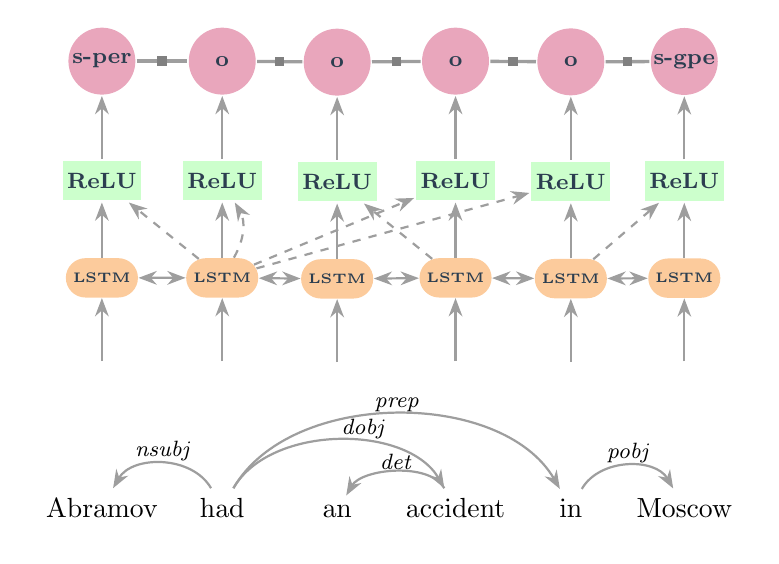
\begin{tikzpicture}[node distance=8.0mm and 10mm, >=Stealth, 
		sentity/.style={draw=none, circle, minimum height=8.5mm, minimum width=8.5mm,line width=1pt, inner sep=0pt, fill=purple!35},
		lstm/.style={draw=none, minimum height=5mm, rounded rectangle, fill=puffin!50, minimum width=11.5mm, label={center:\tiny \textcolor{fontgray}{\bf LSTM}}},
plus/.style={draw=none, minimum height=3mm, circle, fill={rgb:red,0;green,210;blue,211}, label={center:\footnotesize \textcolor{white}{+}}},
		gfunc/.style={draw=none, minimum height=5mm, rectangle, fill=green!20, label={center:\footnotesize \textcolor{fontgray}{\bf ReLU}}, minimum width=10mm, line width = 1.5pt},
		emb/.style={draw=none, minimum height=3mm, rounded rectangle, fill=none, minimum width=12mm, text=fontgray},
chainLine/.style={line width=0.8pt,->, color=mygray},
]
		
		
		\matrix (s) [matrix of nodes, nodes in empty cells, execute at empty cell=\node{\strut};]
		{
			Abramov & [2ex]had & [5ex]an & [3ex]accident   &   [3ex] in  & [3ex] Moscow\\
};
		
		\draw [chainLine, ->] (s-1-2) to [out=120,in=60, looseness=1] node[above, yshift=-1mm, color=black]{\footnotesize\it nsubj} (s-1-1);
		\draw [chainLine, ->] (s-1-4) to [out=120,in=60, looseness=0.8] node[above, yshift=-1mm, color=black]{\footnotesize\it det} (s-1-3);
		\draw [chainLine, ->] (s-1-2) to [out=60,in=120, looseness=0.9] node[above, yshift=-1.2mm, xshift=3mm, color=black]{\footnotesize\it dobj} (s-1-4);
		\draw [chainLine, ->] (s-1-2) to [out=60,in=120, looseness=0.9] node[above, yshift=-1mm, color=black]{\footnotesize\it prep} (s-1-5);
		\draw [chainLine, ->] (s-1-5) to [out=60,in=120, looseness=1] node[above, yshift=-1mm, color=black]{\footnotesize\it pobj} (s-1-6);
		
		\node[emb, above= of s-1-1, yshift=5mm] (u1) {};
		\node[emb, above= of s-1-2, yshift=5mm] (u2) {};
		\node[emb, above= of s-1-3, yshift=5.8mm] (u3) {};
		\node[emb, above= of s-1-4, yshift=5mm] (u4) {};
		\node[emb, above= of s-1-5, yshift=5mm] (u5) {};
		\node[emb, above= of s-1-6, yshift=5mm] (u6) {};
		
		\node[lstm, above= of u1] (h1) {};
		\node[lstm, above=of u2](h2) {};
		\node[lstm, above= of u3](h3) {};
		\node[lstm, above= of u4](h4) {};
		\node[lstm, above= of u5](h5) {};
		\node[lstm, above= of u6](h6) {};
		
		
		
		\node[gfunc, above= of h1, yshift=-1mm] (g1) {};
		\node[gfunc, above=of h2, yshift=-1mm](g2) {};
		\node[gfunc, above= of h3, yshift=-1mm](g3) {};
		\node[gfunc, above= of h4, yshift=-1mm](g4) {};
		\node[gfunc, above= of h5, yshift=-1mm](g5) {};
		\node[gfunc, above= of h6, yshift=-1mm](g6) {};
		




		\node[sentity, above= of g1] (e1) {\footnotesize \textcolor{fontgray}{\bf \textsc{s-per}}};
		\node[sentity, above=of g2](e2) {\footnotesize \textcolor{fontgray}{\bf \textsc{o}}};
		\node[sentity, above= of g3](e3) {\footnotesize \textcolor{fontgray}{\bf \textsc{o}}};
		\node[sentity, above= of g4](e4) {\footnotesize \textcolor{fontgray}{\bf \textsc{o}}};
		\node[sentity, above= of g5](e5) {\footnotesize \textcolor{fontgray}{\bf \textsc{o}}};
		\node[sentity, above= of g6](e6) {\footnotesize \textcolor{fontgray}{\bf \textsc{s-gpe}}};
		
		
		\draw [chainLine] (u1) to (h1);
		\draw [chainLine] (u2) to (h2);
		\draw [chainLine] (u3) to (h3);
		\draw [chainLine] (u4) to (h4);
		\draw [chainLine] (u5) to (h5);
		\draw [chainLine] (u6) to (h6);
		
		\draw [chainLine] (h1) to  (g1);
		\draw [chainLine] (h2) to (g2);
		\draw [chainLine] (h3) to (g3);
		\draw [chainLine] (h4) to (g4);
		\draw [chainLine] (h5) to (g5);
		\draw [chainLine] (h6) to (g6);
		


		\draw [chainLine] (g1) to  (e1);
		\draw [chainLine] (g2) to   (e2);
		\draw [chainLine] (g3) to   (e3);
		\draw [chainLine] (g4) to    (e4);
		\draw [chainLine] (g5) to   (e5);
		\draw [chainLine] (g6) to   (e6);
		
		\draw [chainLine, dashed] (h2) to  [out=60,in=-60] (g2);
		\draw [chainLine, dashed] (h2) to (g1);
		\draw [chainLine, dashed] (h2) to (g4);
		\draw [chainLine, dashed] (h2) to (g5);
		\draw [chainLine, dashed] (h4) to (g3);
		\draw [chainLine, dashed] (h5) to (g6);
		
		\draw [chainLine, <->] (h1) to (h2);
		\draw [chainLine, <->] (h2) to (h3);
		\draw [chainLine, <->] (h3) to (h4);
		\draw [chainLine, <->] (h4) to (h5);
		\draw [chainLine, <->] (h5) to (h6);
		


		\draw [chainLine, line width=1.2pt, -, middlefactor] (e1) to (e2);
		\draw [chainLine, line width=1.2pt, -, middlefactor] (e2)to (e3);
		\draw [chainLine, line width=1.2pt, -, middlefactor] (e3)to (e4);
		\draw [chainLine, line width=1.2pt, -, middlefactor]  (e4)to (e5);
		\draw [chainLine, line width=1.2pt, -, middlefactor] (e5)to (e6);
		
		\end{tikzpicture} 
	}
	\vspace*{-8mm}
	\caption{BiLSTM-GCN-CRF. Dashed connections mimic the dependency edges.}
\label{fig:gcnmodel}
\end{figure}


However, Equation \ref{equ:gcn} does not include the dependency relation information. 
As mentioned in the main paper, such relations have strong correlations with the entity types. 
We modify the Equation \ref{equ:gcn} and include the dependency relation parameter\footnote{The bias vector is ignore for brevity.}:

where  is the dependency relation weight that parameterize the dependency relation  between the -th word and the -th word. 
Such formulation uses the relation to weight the adjacent hidden states in the dependencies. 

\section{Implementation Details}
We implemented all the models with PyTorch~\cite{paszke2017automatic}.
\begin{figure*}[t!]
	\centering
	\includegraphics[width=6.2in]{imgs/gdrelana.eps}
	\caption{Correlations between the entity types and the dependency relation pairs on the grandchild dependencies.}
	\label{fig:gd}
\end{figure*}
For both BiLSTM-CRF and DGLSTM-CRF model, we train them on all datasets with 100 epochs and take the model that perform the best on the development set. 
For BiLSTM-GCN-CRF, we train for 300 epochs with a clipping rate of 3. 


\section{Relation Pairs on Grandchild Dependencies}
Figure \ref{fig:gd} visualized the correlations between the entities and the grandchild dependency relation pairs on the OntoNotes English dataset. 
As mentioned in the paper, such entities are correctly predicted by our models but not the BiLSTM-CRF baseline. 
As we can see from the figure, most of these entities correlate to the ``(\textit{nn}, \textit{nn})'' and ``(\textit{nn}, \textit{pobj})'' relation pairs on the grandchild dependencies. 
Such correlations also show that the relation pair information on the grandchild dependencies can be helpful for detecting certain entities. 



\section{Using Predicted Dependency}

We train a BERT-based~\cite{devlin2019bert} dependency parser~\cite{dozat2017deep} using the training set for each of four languages. 
Specifically, we adopt the \texttt{bert-base-uncased} model for English, \texttt{bert-base-multilingual-cased} for Catalan and Spanish and \texttt{bert-base-chinese} for Chinese.
Because the Chinese BERT model is based on characters but not Chinese words which are segmented. 
We further incorporate a span extractor layer right after BERT encoder for Chinese. 
We following \citet{lee2017end} to design the span extractor layer. Our code for dependency parser is available at \url{https://github.com/allanj/bidaf_dependency_parsing}



\end{document}
